\chapter{Qweak Overall Construction and Layout}\label{CHP_IV}

This class implements the QWeak geometry, including the physical
layout of the components, their material properties and any fields
inside them. The objects and properties currently implemented are
listed in table ~\ref{tbl:IV-I}, together with the respective class
names.  The experimental layout is determined through this class
because the mother volume (experimental hall) is defined here and all
other components are placed inside it and with respect to its origin.
The properties for the individual components are defined in their
respective classes.

\begin{table}
\begin{center}
\begin{tabular}{ll}
\hline 
 {\bf Object / Property} &  {\bf Class}                 \\
\hline 
 Material Type           &  QweakSimMaterial            \\
 Magnetic Field          &  QweakSimMainMagnet          \\
 Target                  &  QweakSimTarget              \\
 Vertical Drift Chambers &  QweakSimVDC                 \\
 Cerenkov Detectors      &  QweakSimCerenkovDetector    \\
 Main Shielding Wall     &  QweakSimCerenkovDetector    \\
\hline
\end{tabular}
\end{center}
\caption{List of experiment components and their classes which are
         currently implemented in the simulation.}
\label{tbl:IV-I}
\end{table}

Aside from the constructor and destructor, there are 5 public access
member functions declared in the header.  In the order they are shown
in fig.~\ref{fig:IV-1} (lines 48 trough 52), they provide a mechanism
to construct the geometry (called by the run manager), they provide
access to the private data members which specify the size of the world
volume (the top most volume), and the last one provides a way to change
the geometry between runs, using the {\em *.mac} file.

\clearpage
\begin{figure}[ht]
  \hspace{0cm}
  \includegraphics[scale=0.8]{./figures4/QweakSimDetectorConstruction.hh-p1.eps}
  \caption{QweakSimDetectorConstruction Header File}
           \label{fig:IV-SC-1}
\end{figure}
\clearpage

\begin{figure}[ht]
  \hspace{0cm}
  \includegraphics[scale=0.8]{./figures4/QweakSimDetectorConstruction.hh-p2.eps}
  \caption{QweakSimDetectorConstruction Header File}
           \label{fig:IV-SC-2}
\end{figure}
\clearpage

\begin{figure}[ht]
  \hspace{0cm}
  \includegraphics[scale=0.8]{./figures4/QweakSimDetectorConstruction.hh-p3.eps}
  \caption{QweakSimDetectorConstruction Header File}
           \label{fig:IV-SC-3}
\end{figure}
\clearpage

\begin{figure}[ht]
  \hspace{0cm}
  \includegraphics[scale=0.8]{./figures4/QweakSimDetectorConstruction.cc-p1.eps}
  \caption{QweakSimDetectorConstruction Source File}
           \label{fig:V-SC-5}
\end{figure}
\clearpage

\begin{figure}[ht]
  \hspace{0cm}
  \includegraphics[scale=0.8]{./figures4/QweakSimDetectorConstruction.cc-p2.eps}
  \caption{QweakSimDetectorConstruction Source File}
           \label{fig:V-SC-6}
\end{figure}
\clearpage

\begin{figure}[ht]
  \hspace{0cm}
  \includegraphics[scale=0.8]{./figures4/QweakSimDetectorConstruction.cc-p3.eps}
  \caption{QweakSimDetectorConstruction Source File}
           \label{fig:V-SC-7}
\end{figure}
\clearpage

\begin{figure}[ht]
  \hspace{0cm}
  \includegraphics[scale=0.8]{./figures4/QweakSimDetectorConstruction.cc-p4.eps}
  \caption{QweakSimDetectorConstruction Source File}
           \label{fig:V-SC-8}
\end{figure}
\clearpage

\begin{figure}[ht]
  \hspace{0cm}
  \includegraphics[scale=0.8]{./figures4/QweakSimDetectorConstruction.cc-p5.eps}
  \caption{QweakSimDetectorConstruction Source File}
           \label{fig:V-SC-9}
\end{figure}
\clearpage

\begin{figure}[ht]
  \hspace{0cm}
  \includegraphics[scale=0.8]{./figures4/QweakSimDetectorConstruction.cc-p6.eps}
  \caption{\label{QweakSimDetectorConstruction} QweakSimDetectorConstruction Source File}
           \label{fig:V-SC-10}
\end{figure}
\clearpage

\begin{figure}[ht]
  \hspace{0cm}
  \includegraphics[scale=0.8]{./figures4/QweakSimDetectorConstruction.cc-p7.eps}
  \caption{QweakSimDetectorConstruction Source File}
           \label{fig:V-SC-11}
\end{figure}
\clearpage

\begin{figure}[ht]
  \hspace{0cm}
  \includegraphics[scale=0.8]{./figures4/QweakSimDetectorConstruction.cc-p8.eps}
  \caption{QweakSimDetectorConstruction Source File}
           \label{fig:V-SC-12}
\end{figure}
\clearpage

\begin{figure}[ht]
  \hspace{0cm}
  \includegraphics[scale=0.8]{./figures4/QweakSimDetectorConstruction.cc-p9.eps}
  \caption{QweakSimDetectorConstruction Source File}
           \label{fig:V-SC-13}
\end{figure}
\clearpage
